%pictures and spectra
%tables and graphs
%statements of the result

%%% three subfigures next to each others
% \begin{figure*}
%     \centering
% \begin{subfigure}{.3\textwidth}
%     \centering
%     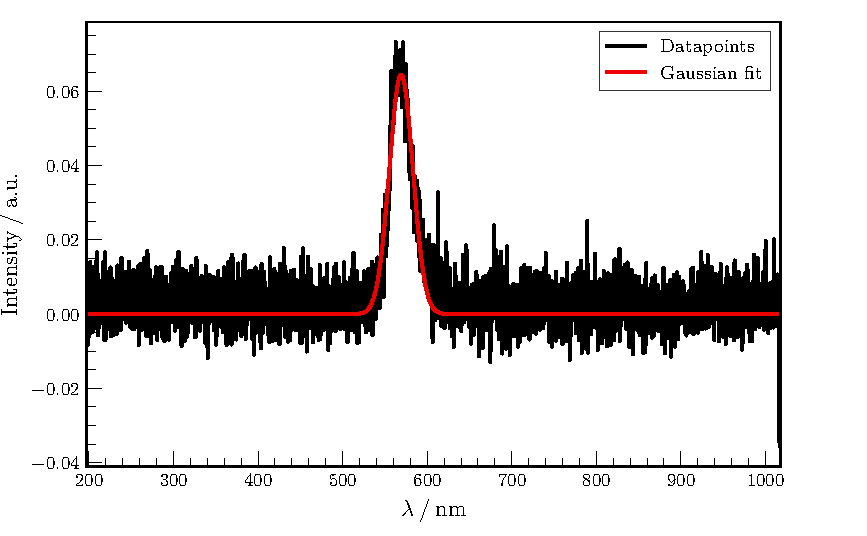
\includegraphics[width=\textwidth]{plots/LED-Green.pdf}
%     \caption{Green LED lightsourse}
%     \label{fig:LEDG}
% \end{subfigure}
% \begin{subfigure}{.3\textwidth}
%     \centering
%     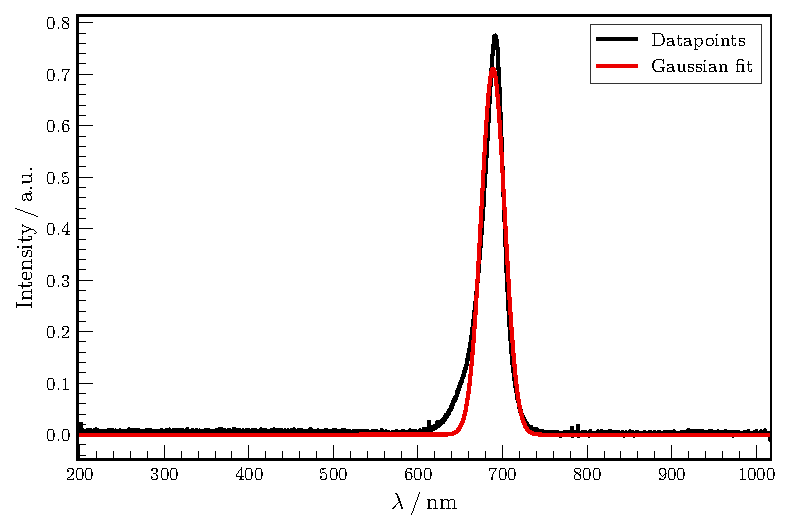
\includegraphics[width=\textwidth]{plots/LED-Red.pdf}
%     \caption{Red LED lightsourse}
%     \label{fig:LEDR}
% \end{subfigure}
% \begin{subfigure}{.3\textwidth}
%     \centering
%     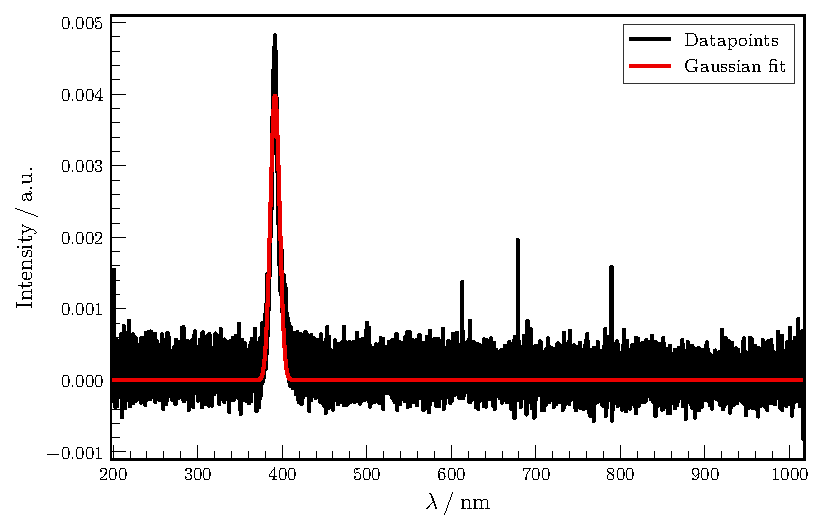
\includegraphics[width=\textwidth]{plots/LED-UV.pdf}
%   \caption{UV LED lightsourse}
%     \label{fig:LEDUV}
% \end{subfigure}
% \caption{Spectral measurement of different LED lightsourse. A Gaussian fit is implemented around the emmision peak.}
% \end{figure*}

%%one figure inside the collums
% \begin{figure}
%     \captionsetup{width=0.9\linewidth}
%     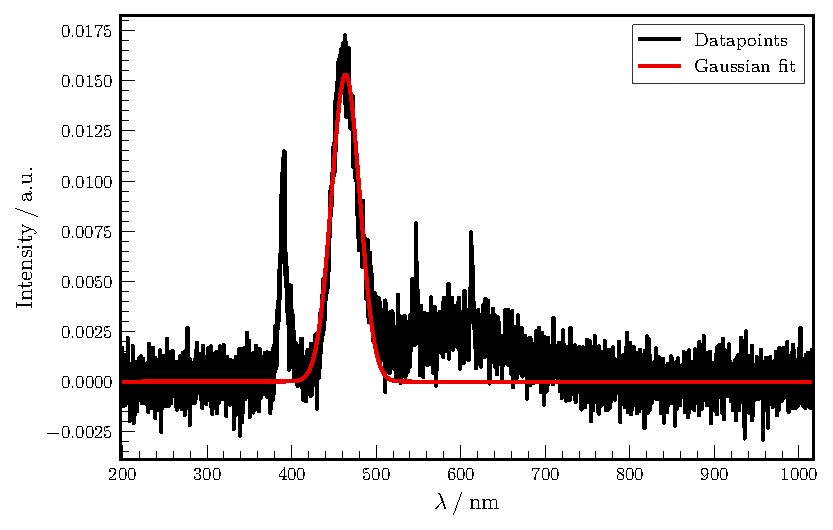
\includegraphics[width=0.5\textwidth]{plots/Samp_A_D.pdf}
%   \caption{Spectral measurement of sample A, excited by a UV-LED lightsource. A Gaussian fit of the peak contributed by luminescense is implemented.}
%     \label{fig:Samp_A_D}
% \end{figure}

\section{Results}
\label{sec:Results}




